\subsection{The model for the vapor pressure}
\indent In this greenhouse climate model, the greenhouse functions heating, insulation, shading, cooling, \ch{CO2} enrichment, humidification and de-humidification are fulfilled by one or more techniques such as a direct air heater, a boiler, an industrial heat source, a geothermal source and passive buffer.\\
\indent For the improvement of a model-based plan strategy, these strategies are viewed as adequately nonexclusive for a wide scope of areas everywhere on the world. Explicit nearby answers for energy creation, energy change or atmosphere adjustment, for example,  co-generation  of  heat  and  electricity,  artificial  photosynthetic  lighting,  an  active heat buffer, a heat pump and a solar heat collector, lie outside the scope of this study. \\
\begin{center}
    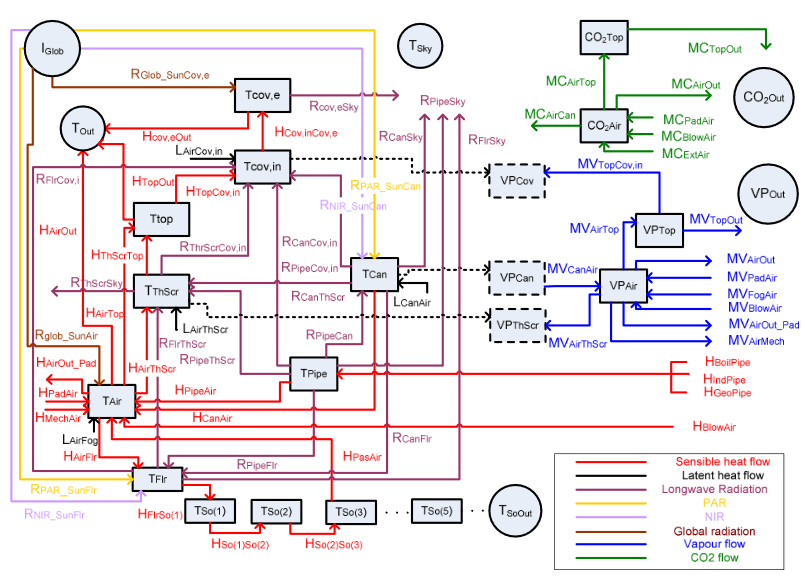
\includegraphics[width=14cm]{Image/Fi2.png}
    \captionof{figure}{\itshape{Overview of the state variables (blocks), semi-state variables (dotted blocks), external climate inputs (circles) and fluxes (arrows) of the greenhouse model. Coloured arrows represent the various energy and mass fluxes (legend at the bottom right).}}    
\end{center}
\indent Thank to De Zwart (1996), this model was based on the greenhouse climate modelling study of him. This model was added some extra elements and parts because of the current purpose.The following model elements were implemented: the design elements presented below in Figure 3. A  lumped  cover  description  to  combine  the  impact  of different  cover  layers  on  indoor  climate;  the  internal  and  external  cover  temperature  are state variables of the model to describe the impact of cover insulation on indoor climate; a description  of  the  far  infrared  radiation  (FIR)  transmission  through  the  cover,  which  is needed for films that partially transmit FIR; a description of both roof and side ventilation; a  description  of  the  impact  of  insect  screens  on  ventilation  rate;  and  a  description  of  the near  infrared  radiation  (NIR)  absorption  of  both  canopy  and  floor,  which  depend  on  the optical  properties  of  the  cover  and  floor.Since optimization of the greenhouse structure properties, i.e. greenhouse dimensions, roof slope and vent orientation and location, exceeded the purpose of our design method,
the model was simplified by not distinguishing between diffuse and direct solar radiation and by assuming that the greenhouse cover transmission coefficient was independent on solar angle.
\begin{center}
    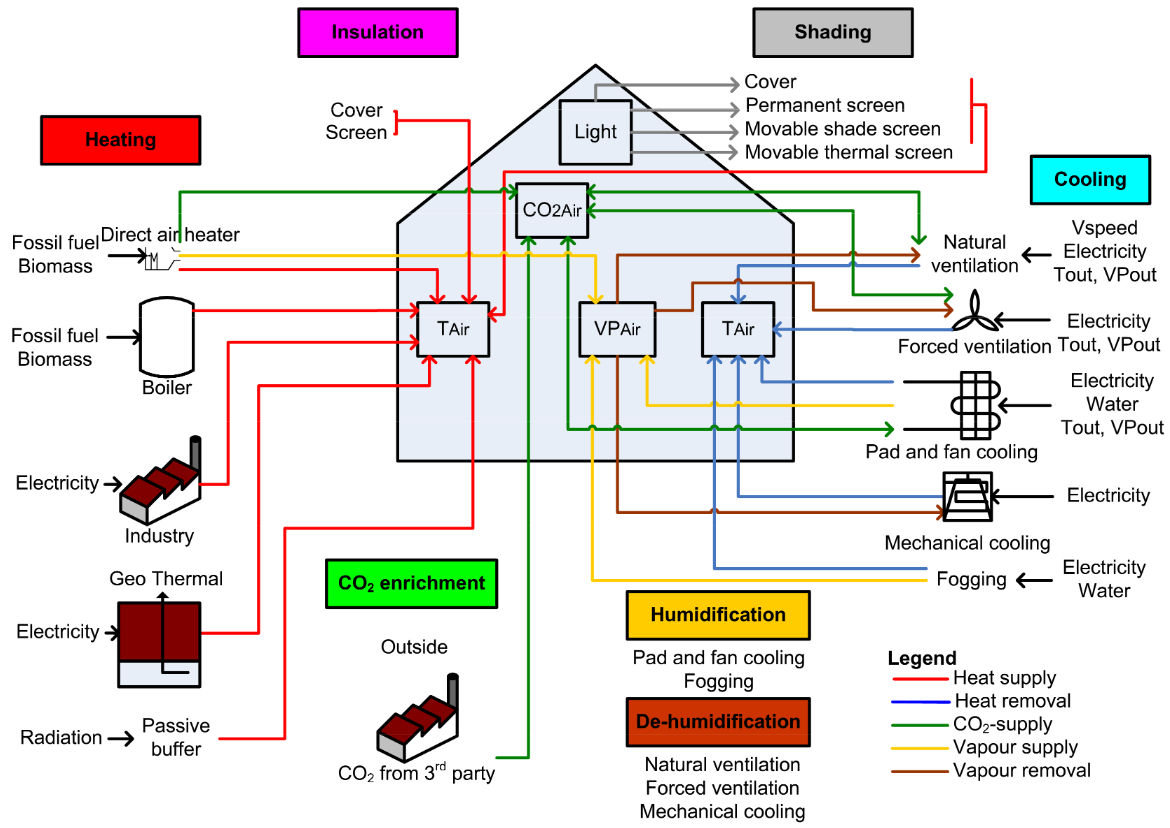
\includegraphics[width=14cm]{Image/Fi1.png}
    \captionof{figure}{\itshape{Selected functions (coloured boxes), and design elements (text blocks and pictures below the accompanying  functions),  needed  for  the  greenhouse design  method  to  manage  the  greenhouse climate (transparent boxes inside the greenhouse). The coloured arrows represent the various energy and mass fluxes (legend at the bottom right).}}    
\end{center}
\indent An overview of the states, the energy and mass fluxes of the greenhouse model is presented in Figure 2 above. This model is based on the following assumptions:
\begin{itemize}
    \item Greenhouse air is considered to be a "perfectly stirred tank" which means that no spatial differences in temperature, vapor pressure and the \ch{CO2} concentration occur. Therefore all the model fluxes are described per square metre of greenhouse floor.
    \item Describing the effect of the thermal screen on the indoor climate, the greenhouse air is divided into compartments: one below and one above the thermal screen.
\end{itemize}
\indent The conditions of the model are totally portrayed by differential conditions. The time subordinates of the states to time are introduced by a dab over the state image. All images are characterized in the Nomenclature.
\subsection{Programs calculate the net \ch{CO2} flux}
The two main equation to calculate the vapor pressure concentration in the lower and upper compartments is

\begin{equation}
\begin{array}{r}
cap_{VP_{Air}}\Dot{VP_{Air}}=MV_{CanAir}+MV_{PadAir}+MV_{FogAir}+MV_{BlowAir}-MV_{AirThScr} \\
-MV_{AirTop}-MV_{AirOut}-MV_{Airout_Pad}-MV_{AirMech}
\end{array}
\end{equation}
\begin{equation}
\begin{array}{r}
cap_{VP_{Top}}\Dot{VP_{Top}}=MV_{AirTop}-MV_{TopCov,in}-MV_{TopOut}
\end{array}
\end{equation}
However, in our model only has:
\begin{equation}
\begin{array}{r}
MV_{CanAir}=-VEC_{CanAir}(VP_{Can}-VP_{Air})
\end{array}
\end{equation}
\begin{equation}
\begin{array}{r}
VEC_{CanAir}=\frac{2\rho_{Air}c_{p.Air}LAI}{\Delta H\gamma (r_{b}+r_{s})}
\end{array}
\end{equation}

\indent Since the canopy temperature was not measured, it was assumed to be equal to the greenhouse air temperature.\\
\begin{center}
\begin{tabular}{m{7cm}m{5.5cm}m{2.5cm}}
 Density of air at sea level: & $\rho_{Air}=1.20$ & $kg m^{-3}$ \\ 
 Specific heat capacity of the air: & $c_{p.Air}=1*10^{-3}$ & $JK^{-1}kg^{-1}$ \\  
 Latent heat of evaporation: & $\Delta H=2.45*10^{6}$ & $Jkg^{-1}water$\\    
 Stefan BoltzMann constant: & $\sigma=5.670*10{-8}$ & $Wm^{-2}K^{-4}$\\    
 Psychrometric constant: & $\gamma=65.8$ & $PaK^{-1}$\\    
 Boundary layer resistance of the canopy for vapor transport: & $r_{b}=275$ & $sm^{-1}$\\
 Stomatal resistance of the canopy: & $r_{s}=r_{s.min}.rf(R_{Can}).$ & \\
  & $rf(CO_{2Air_ppm}.rf(VP_{Can}-VP_{Air})$ &$sm^{-1}$\\
 The minimum canopy resistance for transpiration : & $r_{s.min}=82.0$ & $sm^{-1}$\\  
\end{tabular}
\end{center}
 \indent \indent \indent \indent \indent \indent \indent \indent$rf(R_{Can})=\frac{R_{Can}+c_{evap1}}{R_{Can}+c_{evap2}}$ \\
 \indent \indent \indent \indent \indent \indent \indent$rf(CO_{2Air}=1+c_{evap3}(\eta_{mg_{ppm}CO_{2Air}-200)^{2}}$ \\
 \indent \indent \indent \indent \indent \indent \indent$rf(VP_{Can}-VP{Air}=1+c_{evap4}(VP_{Can}-VP_{Air})^{2}$ \\
\begin{center}
\begin{tabular}{m{7.5cm}m{3cm}m{2.5cm}}
Coefficient of the stomatal resistance model to account for radiation effect&$c_{evap1}=4.30$& $Wm^{-2}$\\
Coefficient of the stomatal resistance model to account for radiation effect&$c_{evap2}=0.54$& $Wm^{-2}$\\
Coefficient of the stomatal resistance model to account $CO_{2}$ effect&$c_{evap3}^{day}=6.1*10{-7}$   $c_{evap3}^{night}=1.1*10{-11}$& $ppm^{-2}$\\
Coefficient of the stomatal resistance model to account for vapor pressure difference&$c_{evap4}^{day}=4.3*10{-6}$ $c_{evap4}^{night}=5.2*10{-6}$& $Pa^{-2}$\\

\end{tabular}
\end{center}
\indent The general form of a vapour flux accompanying an air flux is described by:
\newline
$MV_{12}=\frac{M_{Water}}{R}f_{12}(\frac{VP_{1}}{T_{1}+273.15}-\frac{VP_{2}}{T2+273.15}$ \indent $kgm^{-2}s^{-1}$\\
\indent where $MV_{12}$ is the vapor flux from location 1 to location 2, $f_{12}(m^{3}m^{-2}s^{-1})$ is the air flux from location 1 to location 2, $T_{1}$($^{o}{C}$) is the temperture at location 1 and $T_{2}$($^{o}{C}$) is the temperature at location 2.
\indent The vapor fluxes $MV_{AirTop}$, and $MV_{TopOut}$ are described above analogously. Where by their accompanying air fluxes are $f_{ThScr}$ (the flux through the thermal screen), $f_{VentRoof}$ (flux due to roof ventilation) respectively. We have $VP_{Top}$ and $VP_{Air}$ as input, while $VP_{Out}=1.0$\\
$f_{ThScr}=U_{ThScr}K_{ThScr}|T_{Air}-T_{Out}|^{0.66}+\frac{1-U_{ThScr}}{\rho_{Air}^{Mean}}(0.5\rho_{Air}^{Mean}(1-U_{ThScr})g|\rho_{Air}-\rho_{Out}|)^{0.5}$\\
$K_{ThScr}=0.0002$5\indent $\rho_{Air}^{Mean}=2.99$ \indent \indent $m^{3}m^{-2}s^{-1}$\\
\indent The density of the air is elevation dependent and by assuming a mean air temperature of $20^{o}C$ the density of the air is calculated by:\\
$\rho_{Air}=\rho_{Air0}exp(\frac{gM_{Air}h_{Elevation}}{293.15R})$ \indent \indent $kgm^{-3}$\\
\indent Density of air at sea level $\rho_{Air0}=1.20kgm^{-3}$ and $h_{Elevation}=1470(m)$\\
\indent Molar mass of air: $M_{Air}=28.96 kgkmol^{-1}$\\
\indent $R (Jkmol^{-1}K^{-1})$ is the molar gas constant $g=9.81$
\begin{equation}
f_{\text {VentRoof}}=\left\{\begin{array}{l}
\eta_{\text {Ins}Scr} f_{\text {VentRoof}}^{\prime \prime}+0.5 f_{\text {leakage}}\indent \indent \indent \indent \indent \indent \indentif\eta{roof} \geq \eta_{Roof_Thr}\\
\eta_{\text {Ins}Scr}\left[U_{\text {ThScr}} f_{\text {VentRoof}}^{\prime \prime}\right. \\
\left.+\left(1-U_{\text {ThScr}}\right) f_{VentRoofSide}^{\prime \prime} \eta_{\text {Side }}\right]+0.5 f_{\text {leakage}}\indent if \eta_{Roof}<\eta_{Side_Thr} \\
\indent \indent \indent \indent \indent \indent\indent \indent \indent \indent \indent \indent\indent \indent \indent \indent m^{3}m^{-2}s^{-1}
\end{array}\right.
\end{equation}
\indent The natural ventilation  rate due to roof ventilation is described by Boulard and Baille (1995):
$f_{VentRoof}^{\prime \prime} = \frac{U_{Roof}A_{Roof}C_{d}}{2A_{Flr}}\sqrt{\frac{gh_{Vent}}{2}\frac{T_{Air}-T_{Out}}{T+273.15}+C_{w}v_{Wind}^{2}}$ \indent $m^{3}m^{-2}s^{-1}$\\
\indent $\eta_{Roof_Thr}=0.9$ is the ration between the roof vent area and total ventilation are above no chimney effect and was assumed.
\indent Our model $\eta_{Roof}=1$ since we only have top roof vent, and no insect screen to reduce ventilation rate: $f_{VentRoof}=f_{VentRoof}^{\prime \prime}+0.5f_{leakage}$\\
\indent Furthermore the ventilation rate of the greenhouse is influenced by the greenhouse leakage rate which depends on wind speed and is described by:\\
\begin{equation}
f_{\text {leakage}}=\left\{\begin{array}{l}
0.25*c_{leakage}, \indent v_wind < 0.25 \indent \indent m^{3}m^{-2}s^{-1}\\
c_{leakage*v_{wind}}, \indent v_{wind} \geq 0.25
\end{array}\right.
\end{equation}
\indent Because our $v_{wind}=0.29$ so we $2nd$ formula: $c_{leakage}*v_{wind}$, where $c{leakage}=1*10^{-4}$\\
\indent To calculate $A_{Roof}$, we multiply the specific roof ventilation area $A_{Roof}/A_{Flr}=0.18$ to the surface of the greenhouse floor $A_{Flr}=7,8*10^{4} m^{2}$, which result is $14040 (m^{2})$.\\
\indent $C_{d}=C_{d}^{Gh}(1-\eta_{ShScrC_{d}}U_{ShSc})$\\
\indent$C_{w}=C_{w}^{Gh}(1-\eta_{ShScrC_{w}}U_{ShSc})$\\
\indent Where $C_{d}^{Gh}=0.65$ and$C_{w}^{Gh}=0.9$ for Texas model, since we do not have moving shading screen so the parameter that determines the effect of the movable shading screen on the discharge coefficient $\eta_{ShScrC_{d}} = 0$ and ${ShScrC_{w}}=0$. Other needed variables is: $h_{vent}= 0.97$, $T_{Out}= 23.9 C$, $VP_{out}=1.3$, $T_{Air}=6.8$, $VP_{Air}=12.8$.\\